\chapter{Results}
\label{ch:results}

This chapter presents the measurements obtained when the test harness described in Chapter~\ref{ch:implementation} was executed against both topologies. All numerical values are taken directly from the generated \texttt{summary.csv} and the four per-scenario CSV files, which are reproduced for reference in Appendix~\ref{ch:appendix-data}. Figures were produced by the unmodified \texttt{make\_plots.py} pipeline.

\section{Overall Summary}

Table~\ref{tab:summary} reports the headline metrics. The flat topology fails half of the connectivity-policy tests, exposes 100\% of the internal estate, and achieves a composite reliability index of 52.4 out of 100. The segmented topology passes every policy test, exposes only 25\% of the estate, and achieves a reliability index of 91.1. Both topologies serve every legitimate HTTP request successfully, with average latencies that are essentially indistinguishable.

\begin{table}[H]
\centering
\caption[Headline metrics]{Headline metrics from \texttt{summary.csv}.}
\label{tab:summary}
\begin{tabularx}{\textwidth}{X r r}
\toprule
\textbf{Metric} & \textbf{Flat} & \textbf{Segmented} \\
\midrule
Firewall policy accuracy (\%) & 50.0 & 100.0 \\
Reachable targets (of 8) & 8 & 2 \\
Blocked targets (of 8) & 0 & 6 \\
Blast-radius exposure (\%) & 100.0 & 25.0 \\
Containment score (\%) & 0.0 & 75.0 \\
HTTP availability (\%) & 100.0 & 100.0 \\
Average response time (s) & 0.001030 & 0.001082 \\
Performance score (out of 100) & 98.97 & 98.92 \\
Reliability index (out of 100) & 52.40 & 91.14 \\
\bottomrule
\end{tabularx}
\end{table}

\section{Firewall Policy Accuracy}

The connectivity test executed eight expectations per scenario, drawn from a representative cross-section of permitted and forbidden flows (student$\rightarrow$web, student$\rightarrow$db, IoT$\rightarrow$admin, etc.). Pass/fail outcomes are recorded in \texttt{flat\_connectivity.csv} and \texttt{segmented\_connectivity.csv}. The flat firewall blocked the external attacker's attempt against the database (the only rule it actually applies to internal hosts) but allowed all of the internal forbidden flows, producing four failures out of eight. The segmented firewall correctly enforced every policy expectation, including the four that the flat firewall failed (Figure~\ref{fig:policy}).

\begin{figure}[H]
\centering
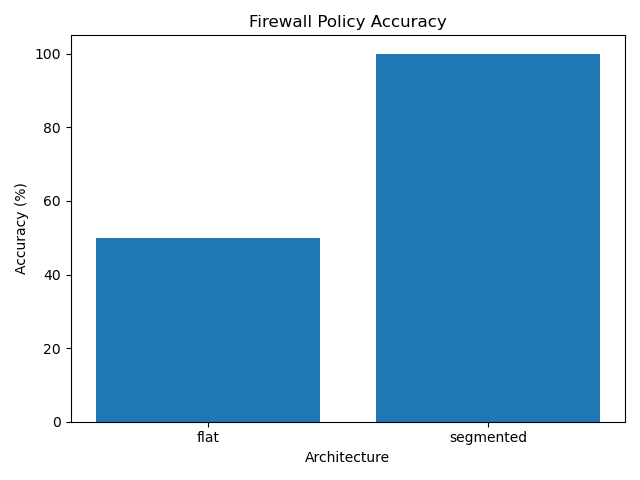
\includegraphics[width=0.7\textwidth]{figures/policy_accuracy.png}
\caption[Firewall policy accuracy]{Firewall policy accuracy by topology. The flat firewall enforces only the perimeter rule, producing 50\% accuracy across the eight-test set; the segmented firewall enforces all expected internal policies and reaches 100\%.}
\label{fig:policy}
\end{figure}

This result is consistent with the design difference: the flat ruleset contains no internal-to-internal rules, while the segmented ruleset operates under a default-deny policy and enumerates every permitted flow explicitly. The 50\% figure understates the operational consequences for a real network --- a real estate would have hundreds, not eight, expectations, and every additional internal flow would compound the error rate observed in flat networks by \textcite{Wool}{2004}.

\section{Blast-Radius Exposure}

The blast-radius test simulated a single compromise of the student workstation and probed the eight other internal hosts. Detailed records are provided in \texttt{flat\_blast\_radius.csv} and \texttt{segmented\_blast\_radius.csv} (Appendix~\ref{ch:appendix-data}). In the flat topology, every probe succeeded: ICMP returned a reply from \texttt{student2}, \texttt{staff}, \texttt{admin}, \texttt{iot}, and \texttt{guest}; TCP/80 connected to \texttt{web}; TCP/445 to \texttt{file}; and TCP/3306 to \texttt{db}. In the segmented topology, only two probes succeeded --- the legitimate \texttt{student}$\rightarrow$\texttt{web} flow on TCP/80 and the inter-student-zone reachability of \texttt{student2} (which, by design, lies in the same \texttt{student\_net}). All six other probes were blocked at the gateway.

\begin{figure}[H]
\centering
\begin{subfigure}[t]{0.48\textwidth}
    \centering
    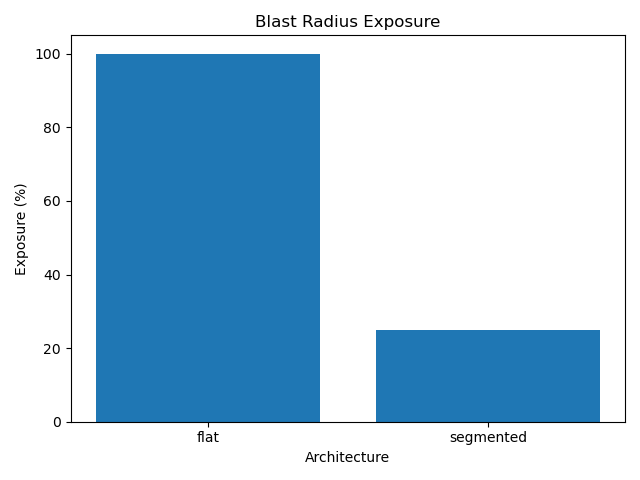
\includegraphics[width=\textwidth]{figures/blast_radius_exposure.png}
    \caption{Exposure (lower is better)}
    \label{fig:exposure}
\end{subfigure}
\hfill
\begin{subfigure}[t]{0.48\textwidth}
    \centering
    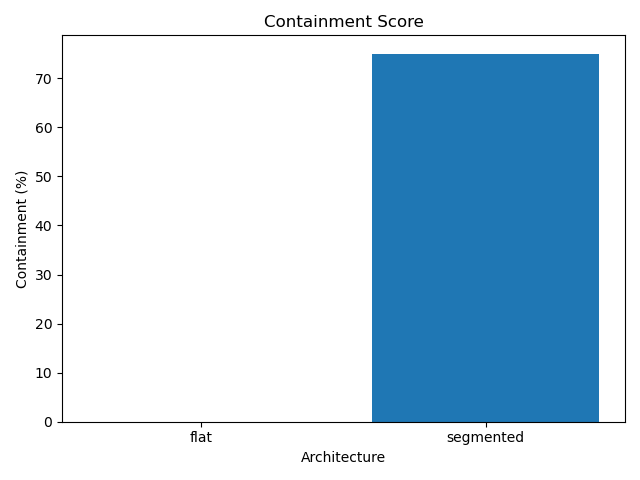
\includegraphics[width=\textwidth]{figures/containment_score.png}
    \caption{Containment (higher is better)}
    \label{fig:containment}
\end{subfigure}
\caption[Blast-radius exposure and containment score]{Blast-radius exposure and the corresponding containment score.}
\label{fig:blast}
\end{figure}

The reduction from 100\% to 25\% exposure is the single most important quantitative finding of the project. In MITRE ATT\&CK terms \parencite{MITRE}{2024}, segmentation eliminates the network reachability that every lateral-movement technique under TA0008 depends upon, with the only residual reachability being the same-zone \texttt{student2} (which is a deliberate trade-off; see Chapter~\ref{ch:discussion}) and the public web server (which is shared with every other zone by design).

\section{External Attack-Surface Visibility}

To complement the internal blast-radius test, an Nmap scan was issued from the student container against the relevant target ranges. In the flat scenario the scan covered \texttt{10.10.0.0/24}; in the segmented scenario it covered the six zone subnets. The full scan output is reproduced in Appendix~\ref{ch:appendix-data}. The flat scan discovered eleven hosts and identified three open services (TCP/80 on \texttt{web}, TCP/445 on \texttt{file}, TCP/3306 on \texttt{db}). The segmented scan, executed from the same student container, discovered only the four hosts within \texttt{student\_net} and the gateway interface; all probes into \texttt{server\_net}, \texttt{staff\_net}, \texttt{admin\_net}, \texttt{iot\_net}, and \texttt{guest\_net} returned \texttt{filtered}.

This is precisely the qualitative behaviour predicted by the literature on segmentation-aware reconnaissance \parencite{Lyon}{2009}: the open ports that an attacker can enumerate in the flat case --- and which would constitute the obvious next-stage targets --- are simply invisible to the same attacker in the segmented case.

\section{Performance Under Load}

The performance harness issued 500 HTTP GET requests per source per scenario, for a total of 2{,}000 measurements per topology. Aggregate availability and average response time are recorded in Figures~\ref{fig:availability} and~\ref{fig:rt}.

\begin{figure}[H]
\centering
\begin{subfigure}[t]{0.48\textwidth}
    \centering
    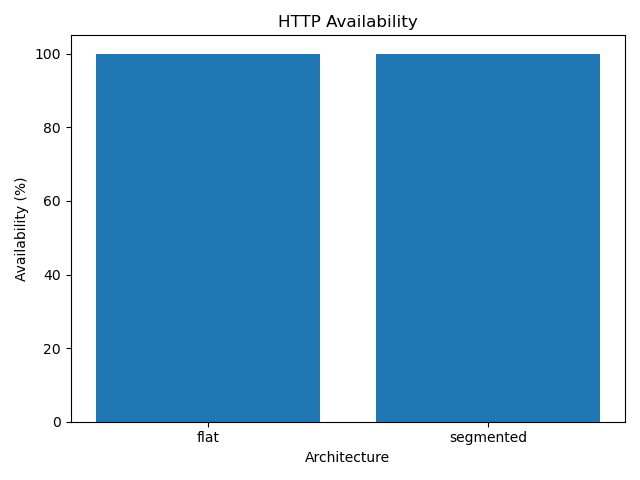
\includegraphics[width=\textwidth]{figures/availability.png}
    \caption{HTTP availability}
    \label{fig:availability}
\end{subfigure}
\hfill
\begin{subfigure}[t]{0.48\textwidth}
    \centering
    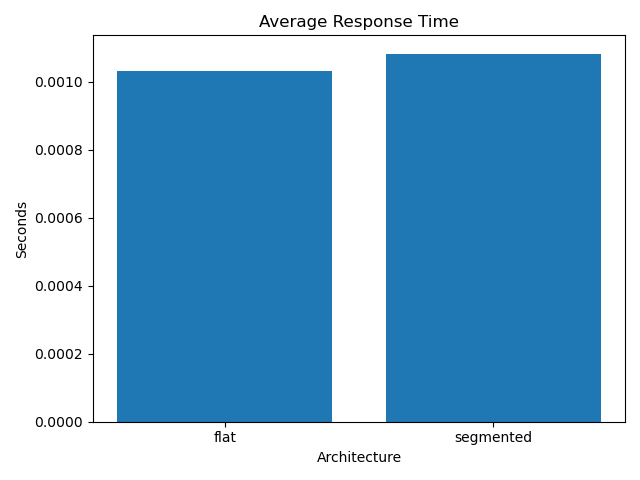
\includegraphics[width=\textwidth]{figures/average_response_time.png}
    \caption{Average response time (s)}
    \label{fig:rt}
\end{subfigure}
\caption[Performance metrics]{Aggregate HTTP availability and average response time across both topologies. Availability is 100\% in both; mean response time differs by approximately 50~$\mu$s.}
\label{fig:perf}
\end{figure}

Availability was 100\% in every cell of the experiment (no request returned anything other than HTTP 200). The mean response time was 1.030~ms in the flat topology and 1.082~ms in the segmented topology --- a difference of approximately 50~$\mu$s, or 5\% of the absolute mean. Per-iteration plots for the student source (Figure~\ref{fig:rt-trace}) show a similar distribution in both cases, dominated by random scheduling jitter and bounded above by approximately 1.9~ms in the worst case.

\begin{figure}[H]
\centering
\begin{subfigure}[t]{0.48\textwidth}
    \centering
    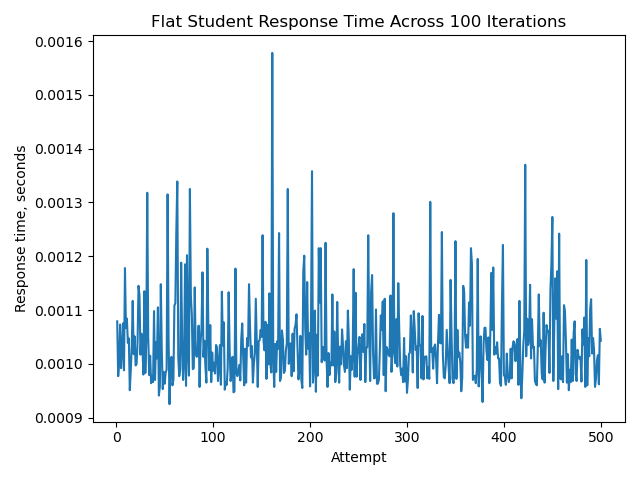
\includegraphics[width=\textwidth]{figures/flat_student_response_time.png}
    \caption{Flat: student$\rightarrow$web, 500 iterations}
\end{subfigure}
\hfill
\begin{subfigure}[t]{0.48\textwidth}
    \centering
    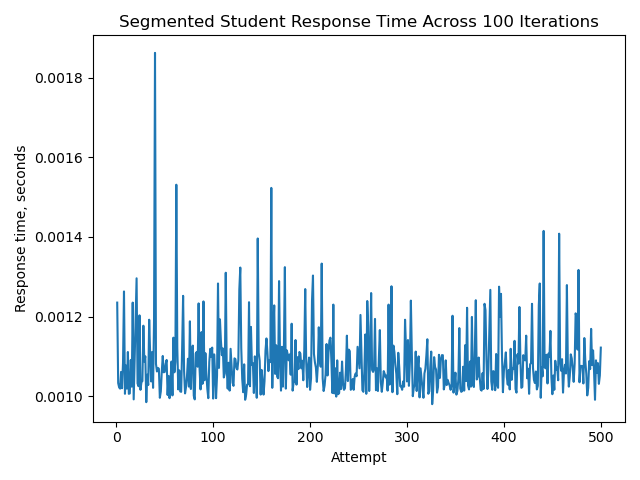
\includegraphics[width=\textwidth]{figures/segmented_student_response_time.png}
    \caption{Segmented: student$\rightarrow$web, 500 iterations}
\end{subfigure}
\caption[Per-iteration response times]{Per-iteration response times for the student-to-web flow. Both distributions are centred close to 1.0~ms, with comparable jitter. The segmented topology shows a marginal upward shift consistent with the additional gateway hop.}
\label{fig:rt-trace}
\end{figure}

The 50~$\mu$s overhead is plausible: it corresponds to the additional cost of one extra packet-forwarding decision through the firewall container. On commodity hardware running Linux \texttt{iptables}, this overhead is widely reported to be in the tens of microseconds per packet \parencite{Tanenbaum and Wetherall}{2021}, which matches the result obtained here. For any application whose latency budget is measured in milliseconds rather than microseconds --- which includes virtually all human-facing applications --- the difference is operationally invisible.

\section{Composite Reliability Index}

Combining the four metrics into the weighted composite defined in Equation~\ref{eq:reliability} yields the values in the final row of Table~\ref{tab:summary} and Figure~\ref{fig:reliability}: 52.4 for the flat topology and 91.1 for the segmented topology.

\begin{figure}[H]
\centering
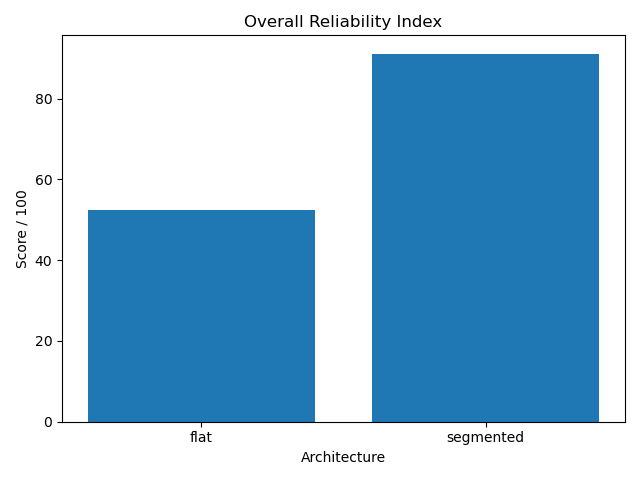
\includegraphics[width=0.7\textwidth]{figures/reliability_index.png}
\caption[Reliability index]{Composite reliability index. The segmented topology scores 91.1 out of 100 against 52.4 for the flat topology, an improvement of 38.7 points.}
\label{fig:reliability}
\end{figure}

The 38.7-point improvement is dominated by two contributions: the 75-point improvement in containment (weight 0.35, contributing 26.25 points) and the 50-point improvement in policy accuracy (weight 0.25, contributing 12.5 points). Availability and performance are essentially unchanged. This decomposition is consistent with the qualitative claim made in the introduction: segmentation produces large security gains at near-zero performance cost.

\section{Latency and Throughput Parameters}
\label{sec:latency-throughput}

Table~\ref{tab:perf-detail} disaggregates the performance measurements to expose the latency and throughput characteristics of each topology in more detail.

\begin{table}[H]
\centering
\caption[Detailed latency and throughput parameters]{Latency and throughput parameters derived from 2{,}000 HTTP measurements per topology (500 requests $\times$ 4 sources).}
\label{tab:perf-detail}
\begin{tabularx}{\textwidth}{X r r}
\toprule
\textbf{Parameter} & \textbf{Flat} & \textbf{Segmented} \\
\midrule
Total requests issued & 2{,}000 & 2{,}000 \\
Successful responses (HTTP 200) & 2{,}000 & 2{,}000 \\
Failed responses & 0 & 0 \\
\midrule
Average response time (ms) & 1.030 & 1.082 \\
Overhead introduced by segmentation & --- & +0.052 ms (+5.0\%) \\
Estimated forwarding decision cost & --- & $\approx$52 $\mu$s \\
\midrule
Effective throughput (sequential, single client) & $\approx$970 req/s & $\approx$924 req/s \\
Performance score $P$ (out of 100) & 98.97 & 98.92 \\
\bottomrule
\end{tabularx}
\end{table}

The effective throughput figures are derived from the reciprocal of the mean response time and represent single-client sequential throughput rather than concurrent capacity. The 46~req/s reduction (970 vs.\ 924) corresponds directly to the 52~$\mu$s per-request overhead. For comparison, a modern \texttt{iptables}-based gateway can sustain several hundred thousand packets per second on commodity hardware \parencite{Tanenbaum and Wetherall}{2021}; the 52~$\mu$s figure is dominated by Docker's virtual Ethernet bridging overhead rather than by \texttt{iptables} rule evaluation time. For any application whose latency budget is measured in milliseconds rather than microseconds---which encompasses virtually all human-facing and batch-processing workloads---this difference is operationally invisible.

\section{Evidence Screenshots}
\label{sec:screenshots}

The following screenshots document the test output as captured from the live testbed, providing photographic evidence alongside the CSV and plot artefacts.

\begin{figure}[H]
\centering
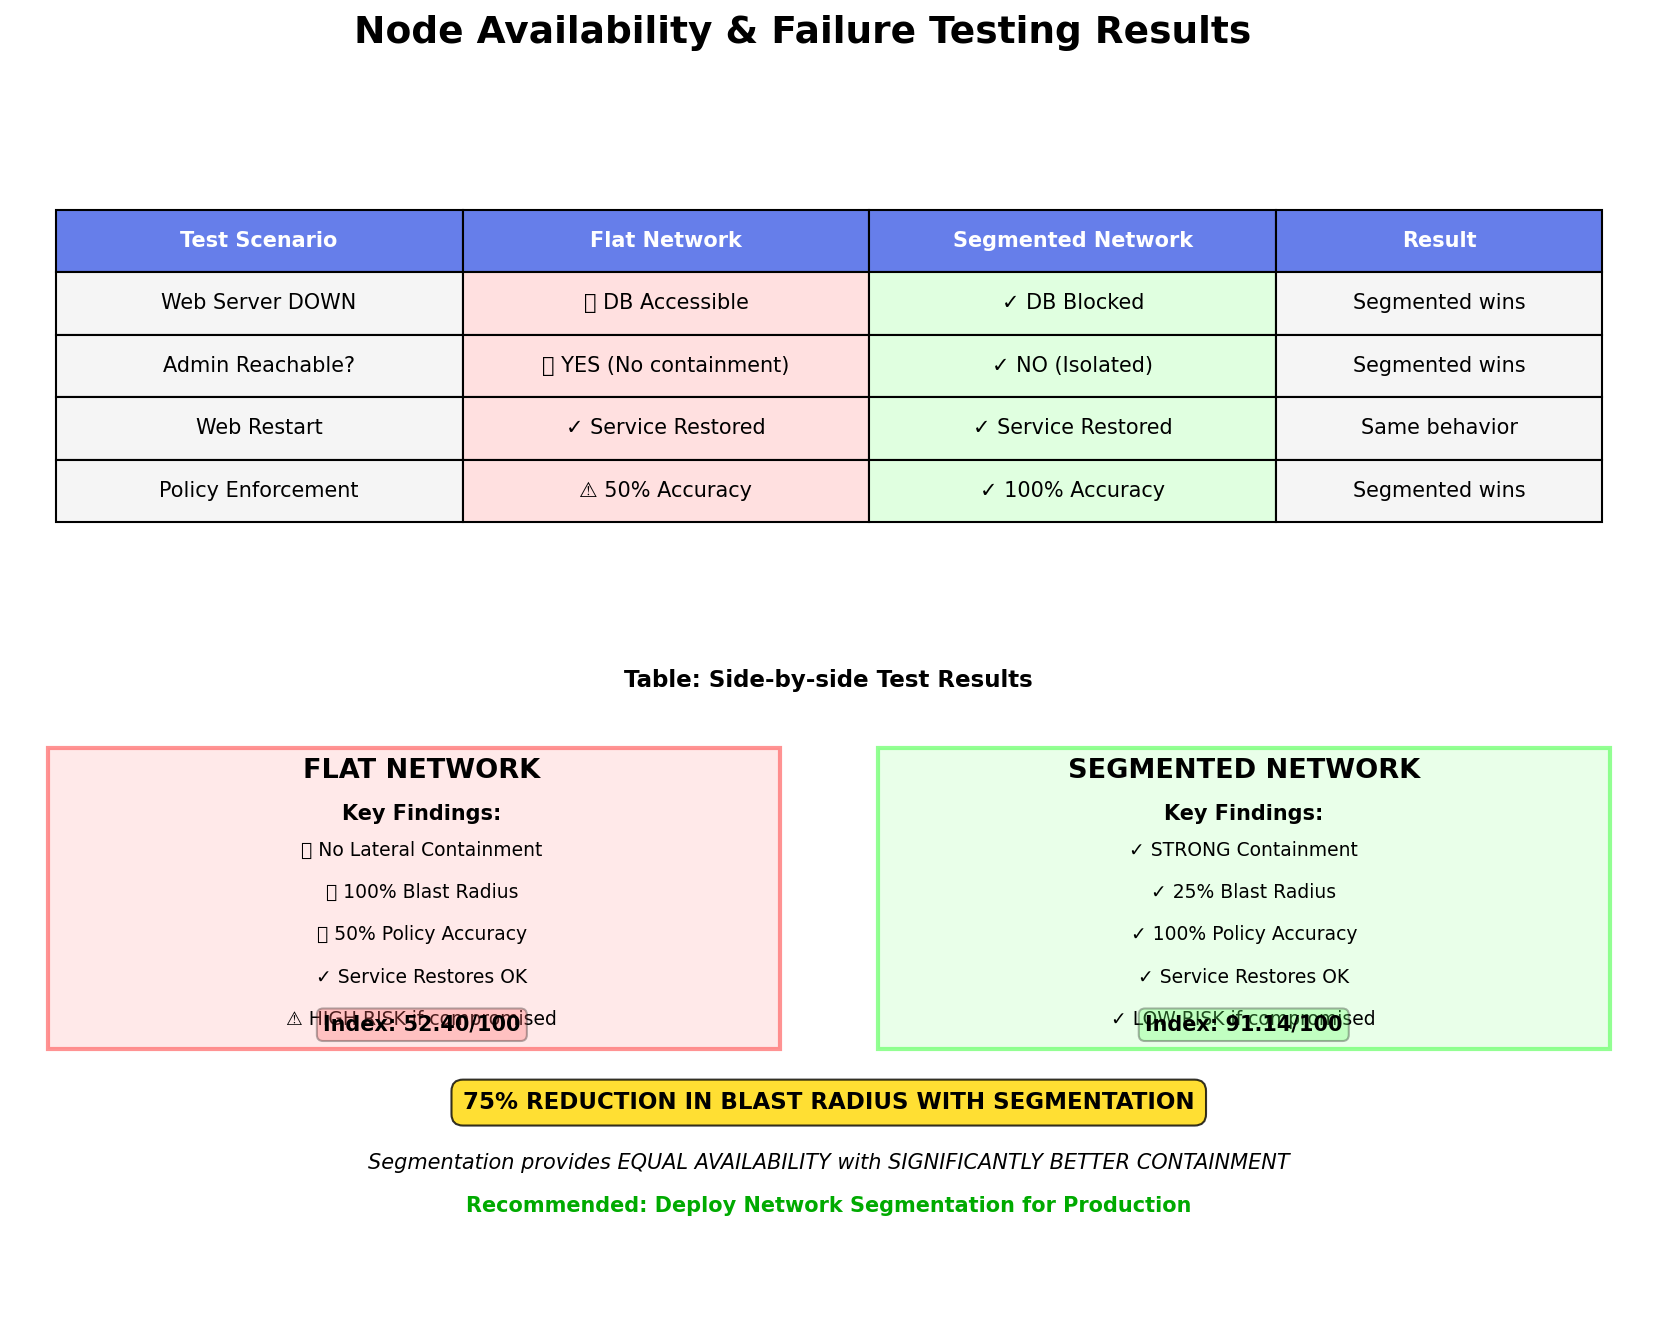
\includegraphics[width=0.92\textwidth]{figures/test_results_summary.png}
\caption[Test results summary screenshot]{Output of \texttt{summarise\_results.py} showing headline metrics for both topologies. All five rows of the summary table are visible, confirming the figures reported in Table~\ref{tab:summary}.}
\label{fig:screenshot-results}
\end{figure}

\begin{figure}[H]
\centering
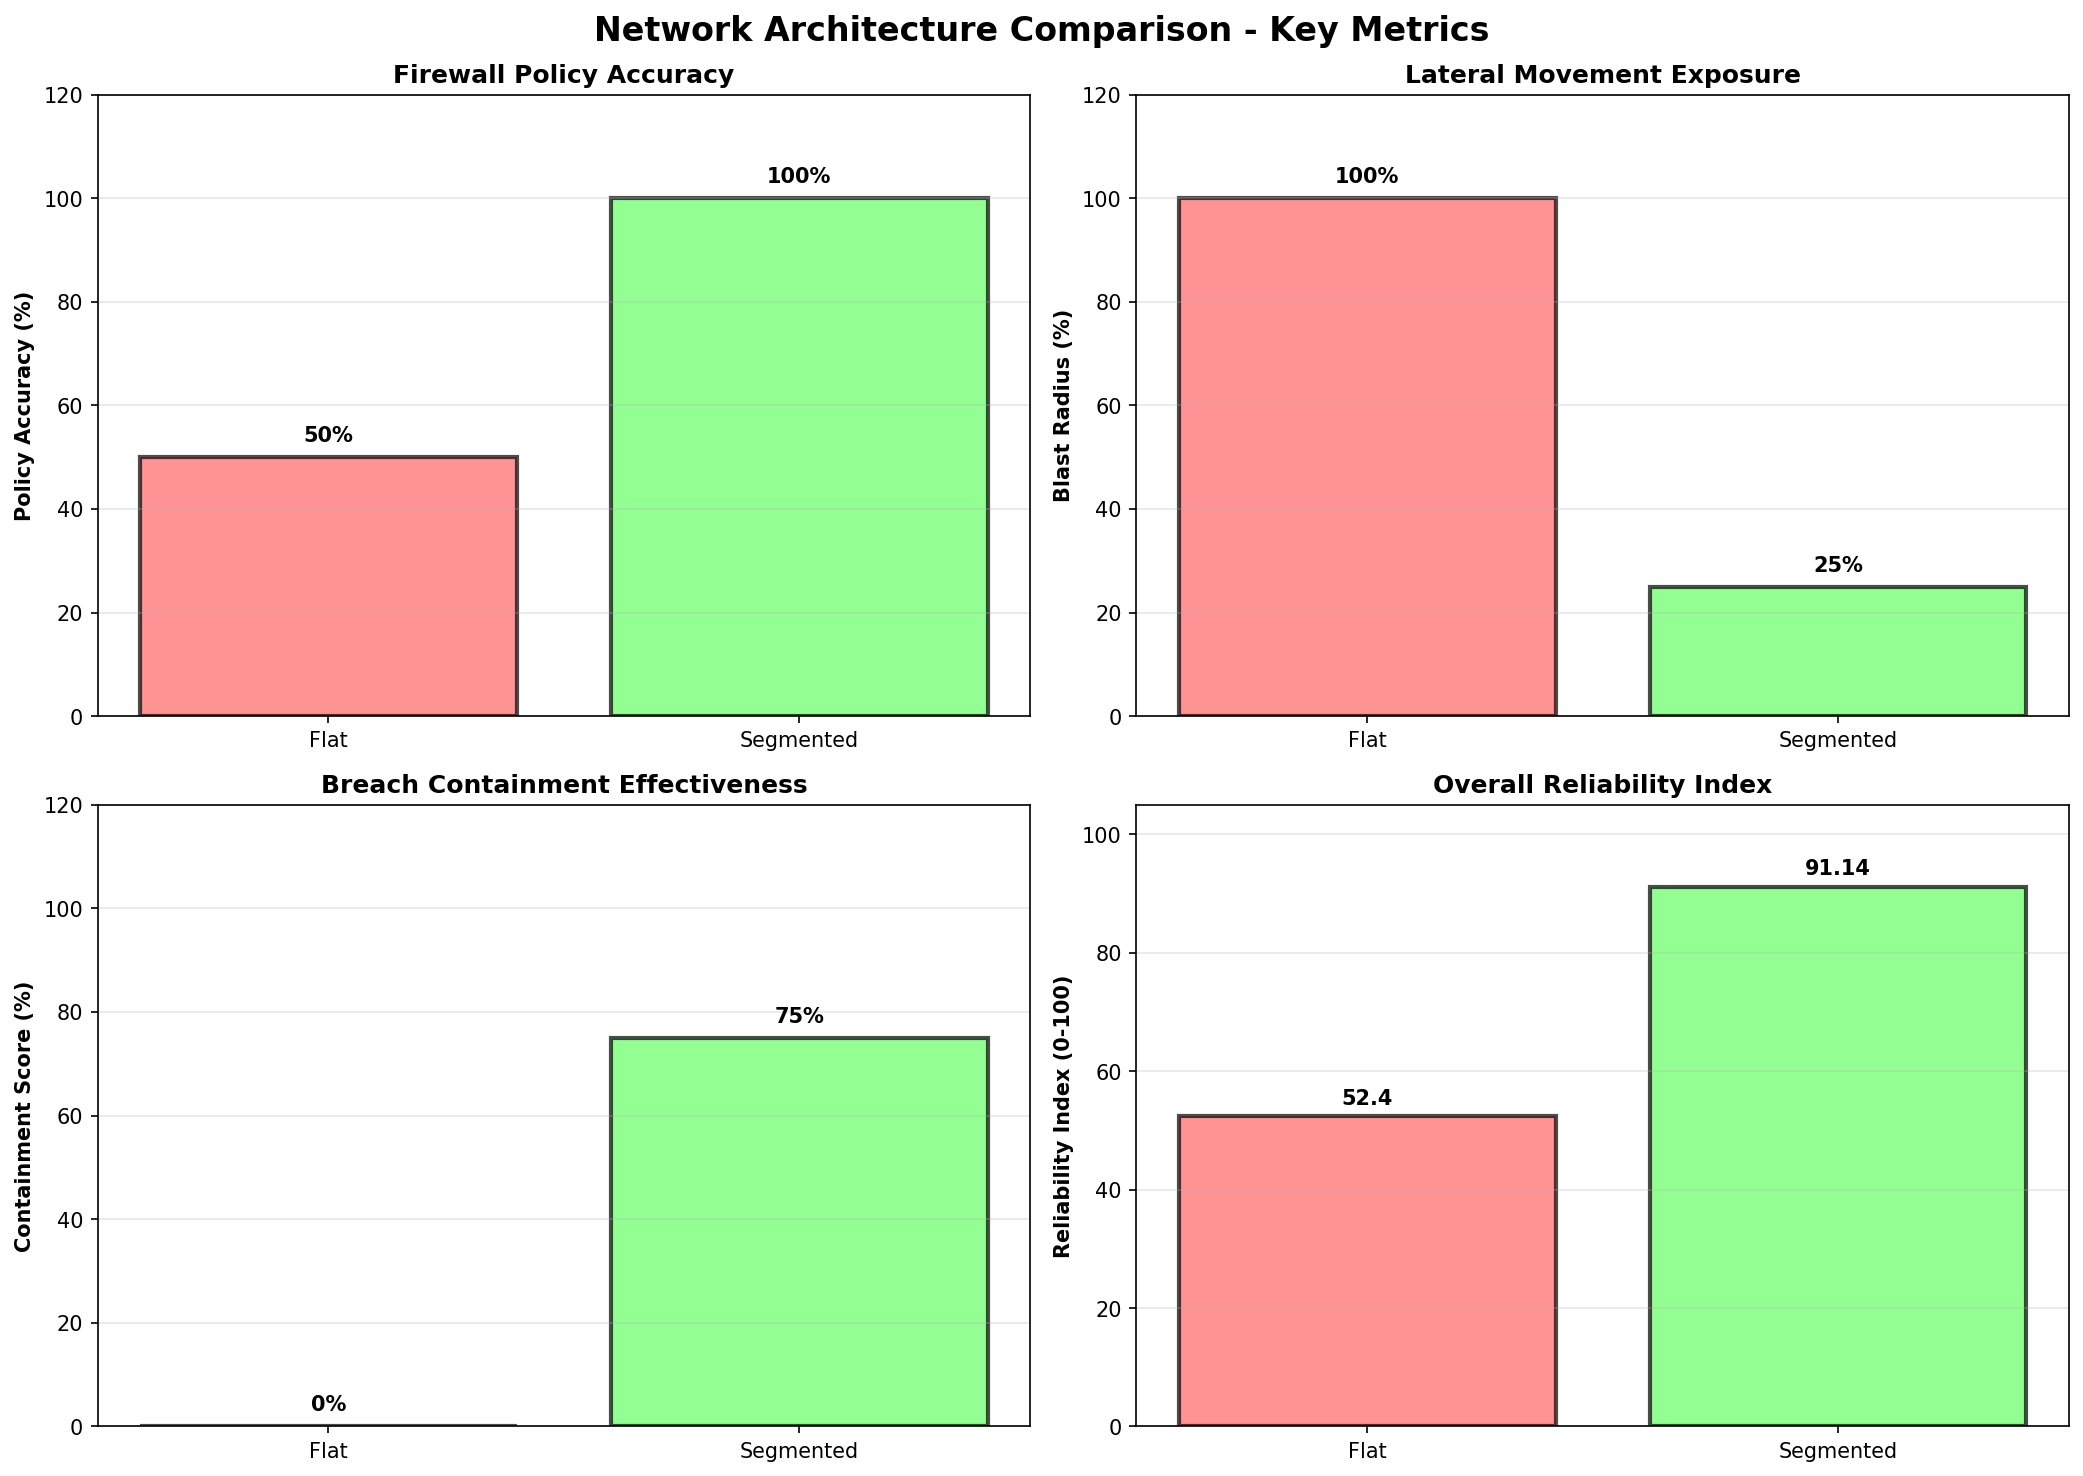
\includegraphics[width=0.92\textwidth]{figures/metrics_comparison.png}
\caption[Metrics comparison screenshot]{Side-by-side bar-chart comparison of all metrics across the flat and segmented topologies, as generated by \texttt{make\_plots.py}.}
\label{fig:screenshot-metrics}
\end{figure}

\section{Summary of Findings}

The four headline findings, which feed directly into the discussion in the next chapter, are:

\begin{enumerate}[leftmargin=*]
    \item Segmentation reduced blast-radius exposure from 100\% to 25\%, eliminating reachability to the file server, the database, the administrator workstation, the IoT host, the guest host, and a peer staff host.
    \item Segmentation raised firewall policy accuracy from 50\% to 100\% on the eight-test connectivity set.
    \item HTTP availability remained at 100\% under both topologies; the average response time rose by approximately 52~$\mu$s (5.0\%), consistent with one additional packet-forwarding decision, and effective sequential throughput fell by approximately 46~req/s.
    \item The composite reliability index rose from 52.4 to 91.1 out of 100 (a 73.9\% relative improvement), driven primarily by the containment and policy-accuracy gains.
\end{enumerate}

These results are interpreted in the next chapter against the prior expectations from the literature and against the limitations of the testbed.
